\documentclass[landscape,spanish]{article}

\usepackage{acronym,amsthm,babel,boxedminipage,longtable,fancyhdr,framed,colortbl,epsfig,lscape,multirow,setspace,tabularx,titlesec,moreverb,xcolor,xspace}

\usepackage[%
bookmarks,bookmarksopen,bookmarksnumbered,bookmarksopenlevel=2,%
%pdfkeywords=Interactive\ Transcription; Interactive\ Translation,%
pdftitle=LLMs,%
citebordercolor=blue,
filebordercolor=teal,
linkbordercolor=lightgray,
menubordercolor=violet,
urlbordercolor=lightgray,
runbordercolor=darkgray]{hyperref}

\usepackage{alltt,amsmath,boxedminipage,calc,datetime,dcolumn,ifthen,moreverb,multido,pifont,psboxit,rotating,tabularx}
\usepackage[utf8]{inputenc}
\usepackage{mllp}
\usepackage{tikz}
\usepackage{amsfonts}
\usepackage{bm}
\usepackage{booktabs}
\usepackage{multicol}
\usepackage[eulergreek]{sansmath}
\usetikzlibrary{arrows,shapes,snakes,automata,backgrounds,petri,calc,fit,positioning}

\graphicspath{{../figures/}{figures/}}

\newcommand{\cmark}{\ding{51}}%
\newcommand{\xmark}{\ding{55}}%

\pagestyle{plain}

\renewcommand{\today}{16 de Julio, 2024}
\renewcommand{\title}{Adaptación de modelos de lenguaje grandes para tareas de traducción automática}
\renewcommand{\author}{Sergio Madrid Pérez}
\renewcommand{\authorshort}{Sergio Madrid Pérez}
\renewcommand{\titleshort}{Adaptación de LLMs para tareas de TA}

\renewcommand\labelitemi{$\bullet$}

%\institute[Universitat Politècnica de València]

%-------------------------------------------------------------------------------
% COLORS:

\definecolor{mygrey}{gray}{.75}
\definecolor{gray}{rgb}{0.9,0.9,0.9}
\definecolor{drakgray}{rgb}{0.34,0.35,0.32}
\definecolor{darkred}{rgb}{0.71,0.13,0.14}
\definecolor{darkgreen}{rgb}{0.2,0.5,0.3}
\definecolor{greygreen}{rgb}{0.25,0.5,0.25}
\definecolor{greyblue}{rgb}{0.34,0.34,0.42}
\definecolor{darkblue}{rgb}{0.1,0.2,0.6}
\definecolor{darkmagenta}{rgb}{.55,0,.55}

%-------------------------------------------------------------------------------
% SUBSUBSUBSECTION:

%\titleformat{\paragraph}{\normalsize\bfseries}{\theparagraph}{1em}{}
%\titlespacing*{\paragraph}{0pt}{3.5ex plus 1ex minus .2ex}{2.3ex plus .2ex}

\setcounter{secnumdepth}{1} % section numbering is applied up to this level
\setcounter{tocdepth}{2} % sections up to given depth are included in toc

\begin{document}

\thispagestyle{empty}

% \begin{center}

% \centerline{
\includegraphics[height=0.15\textheight]{figures/UPV-logo}}

% \rule{0mm}{20mm}
% \Large{\setstretch{1.5}\Large\textbf{\color{darkred}\title}}

% \rule{0mm}{30mm}
% {\normalsize \color{greyblue}\author}

% \newcolumntype{Y}{>{\centering\arraybackslash}X}
% \rule{0mm}{0mm}
% \begin{table}[ht!]
%     \begin{tabularx}{\textwidth}{YYY}
%         \small \color{greyblue} Alfons Juan Císcar & \small \color{greyblue} Jorge Civera Saiz &
%         \small \color{greyblue} Jorge Iranzo Sánchez \\
%     \end{tabularx}
% \end{table}

% \end{center}

% \centerline{
\includegraphics[height=0.12\textheight]{figures/MLLP_Brand} \qquad \qquad 
\includegraphics[height=0.15\textheight]{figures/dsic.jpeg}}

% \normalsize\small
% \vspace{10mm}

% %\centerline{\today}
% \vfill

\begin{center}

	\rule{0mm}{35mm}
	\Large{\setstretch{1.5}\Large\textbf{\color{darkred}\title}}

	\rule{0mm}{30mm}
	{\normalsize \fontsize{22}{20} \textbf{\color{greyblue}\author}}
	\vspace{-10mm}

	\newcolumntype{Y}{>{\centering\arraybackslash}X}
	\rule{0mm}{0mm}
	\begin{table}[ht!]
		\centering
		\begin{tabularx}{\textwidth}{YYY}
			\small \color{greyblue} \textbf{Tutor} &
			\small \color{greyblue} \textbf{Cotutor} &
			\small \color{greyblue} \textbf{Director experimental}\\
		\end{tabularx}
	\end{table}
	\vspace{-15mm}
	\begin{table}[ht!]
		\centering
		\begin{tabularx}{\textwidth}{YYY}
			\small \color{greyblue} Alfons Juan Ciscar & 
			\small \color{greyblue} Jorge Civera Saiz & 
			\small \color{greyblue} Jorge Iranzo Sánchez\\
		\end{tabularx}
	\end{table}
\end{center}

\normalsize\small

% \begin{center}
% 	\today
% \end{center}

\normalsize
\vspace{10mm}

\centerline{\color{greyblue} \today}
\vfill

\vspace{20mm}
\centerline{
	
\includegraphics[height=0.1\textheight]{figures/MLLP_Brand} 
	\qquad 
	\qquad 
	
\includegraphics[height=0.12\textheight]{figures/dsic.jpeg}
}

\vfill

\clearpage %-------------------------------------

\hypertarget{INDEX}{}

%\doublespacing
\tableofcontents
%\singlespacing

\cp %-----------------------------------
\section{Introducción}
\vspace*{10mm}

\subsection*{Motivación}
\vspace*{5mm}
\begin{itemize}\itemsep=5mm
    %\item Beca de colaboración en VRAIN

    %\item Traducción automática (MT) se basa en modelos neuronales (Transformer)

    \item Modelos de lenguaje grandes (LLMs) han revolucionado la IA

    \item LLMs muy exitosos en procesamiento del lenguaje natural (NLP), incluida la traducción automática (MT)

    \item Beca de colaboración en MLLP

\end{itemize}

\subsection*{Objetivos}
\vspace*{5mm}
\begin{itemize}\itemsep=5mm
    \item Evaluar los modelos encoder-decoder más recientes diseñados para TA

    \item Adaptar y evaluar LLMs para TA

    \item Evaluar las capacidades de aprendizaje en contexto de los LLMs para TA

\end{itemize}

\cp %------------------------------------------

\phantomsection
\refstepcounter{section}
\addcontentsline{toc}{section}{\quad\thesection\text{ }\text{ } Fundamentos Teóricos}
\section*{\thesection.\quad Fundamentos: Transformer}
\vspace*{10mm}

% \begin{minipage}{0.4\linewidth}
% \begin{itemize}\itemsep=10mm
%     \item Modelo de aprendizaje profundo compuesto por un encoder y un decoder.

%     \item El mecanismo de atención permite hallar las relaciones entre palabras en una oración.

%     \item Se ha convertido en el modelo de facto para tareas de PLN.


% \end{itemize}
% \end{minipage}
% %
% \begin{minipage}[H]{0.6\textwidth}
% \begin{flushright}
% \centering
% 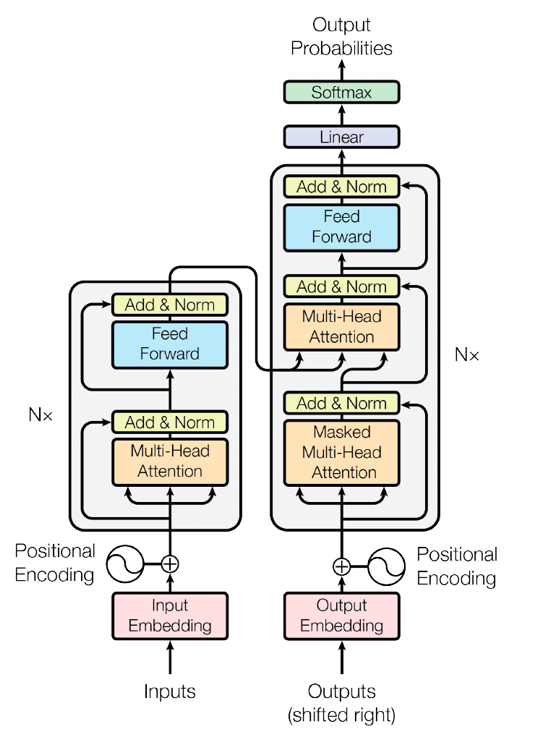
\includegraphics[scale=1]{transformer.png}
% \end{flushright}
% \end{minipage}

\centering
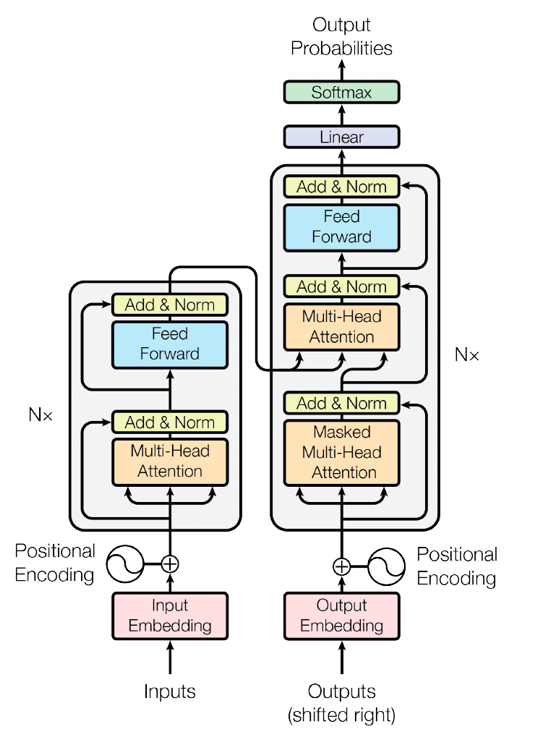
\includegraphics[width=0.4\linewidth]{transformer.png}


\cp %------------------------------------------
\section*{\thesection.\quad Fundamentos: LLMs}
\vspace*{10mm}

\begin{itemize}\itemsep=10mm
    \item  Típicamente decoder de Transformer con gran número de parámetros

    \item  Se entrenan con colecciones de datos muy extensas

    \item  Adaptabilidad a diversas tareas NLP con gran éxito

    \item  Uso de técnicas de ajuste eficiente de parámetros (PEFT) como LoRA

\end{itemize}

\vspace*{10mm}
\centering
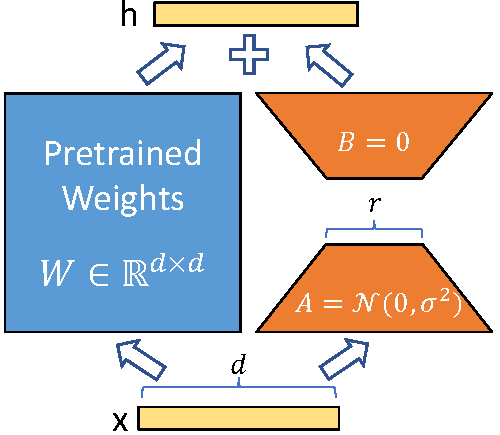
\includegraphics[scale=1.1]{lora.pdf}

\cp %------------------------------------------
\section*{\thesection.\quad Fundamentos: neural MT}
\vspace*{10mm}

\begin{itemize}\itemsep=10mm

    \item Estado del arte: encoder-decoder con atención (Transformer)

    \item Últimos resultados con LLMs comparables con el estado del arte

    \item Métricas de evaluación usuales: BLEU y COMET
\end{itemize}

% \begin{equation*}
% \boldsymbol{\hat{y}} = \argmax_{\boldsymbol{y}}P(\boldsymbol{y} \mid \boldsymbol{x})
% \end{equation*}


\cp %------------------------------------
\refstepcounter{section}
\addcontentsline{toc}{section}{\quad\thesection\text{ }\text{ } Modelos encoder-decoder}
\section*{\thesection.\quad Modelos encoder-decoder: Datasets}
\vspace*{10mm}

\subsection*{Evaluación}
\vspace*{10mm}

\flushleft
\begin{minipage}{0.25\linewidth}
\vspace{-10mm}
\begin{itemize}
    \item INTERACT
    \item Europarl-ST
\end{itemize}
\end{minipage}
%
\begin{minipage}[h]{0.5\linewidth}
    \centering
    Nº de oraciones en cada test set \\
    \vspace{6mm}
	\begin{tabular}{r||cc}
		   %&  \multicolumn{2}{c}{Nº} \\
	       $en \rightarrow$ & INTERACT & Europarl-ST \\ \hline
		   $es$  & 1405 & 1267  \\ 
		   $de$  & 1399 & 1253  \\
	\end{tabular} 
    \label{table:test-datasets}
\end{minipage}

\subsection*{Entrenamiento}
\vspace*{10mm}

\begin{minipage}{0.27\linewidth}
\begin{itemize}
    \item Medline-WMT22
    \item Europarl-ST
    \item MuST-C
\end{itemize}    
\end{minipage}
\begin{minipage}[H]{0.5\linewidth}
    \centering
    \scalebox{1}{
    \begin{tabular}{r||r|r|r}
        \multirow{2}{*}{$en \rightarrow$} & \multirow{2}{*}{Sentences} & \multicolumn{2}{c}{Words} \\
        \cline{3-4}
        & & Source & Target \\
        \hline
        $es$ & 442.5 K & 9.2 M & 9.7 M \\
        $de$ & 361.2 K & 7.1 M & 6.7 M \\
    \end{tabular}
    }
    \label{tab:train_datasets}
\end{minipage}

% \cp %------------------------------------------
% \section{Modelos encoder-decoder para TA}
% \vspace*{10mm}

% \begin{itemize}\itemsep=10mm
%     \item NLLB 600M, 1.3B, 3.3B
    
%     \item Madlad 3B
    
%     \item Helsinki 500M

%     \item Google Translate
% \end{itemize}


\cp %-----------------------------------------
%\section*{\thesection\quad }
\section*{\thesection.\quad Modelos encoder-decoder: INTERACT}
\vspace*{10mm}

\begin{table}[h]
\centering
%\textbf{Resultados de los modelos encoder-decoder en el test set INTERACT: en $\rightarrow$ es, de \\}
%\textbf{Resultados en el test set INTERACT \\}
\vspace*{10mm}
\scalebox{1}{
\begin{tabular}{l c c c c c c}
    \toprule
    {} & {} & \multicolumn{2}{c}{Spanish} & {} & \multicolumn{2}{c}{German} \\ \cmidrule{3-7} 
    Model & LoRA & BLEU & COMET & {} & BLEU & COMET \\
    \midrule \midrule
    Google Translate & No & 56.7 & \textbf{87.6} & {} & 40.5 & \textbf{86.5} \\ 
    %\midrule
    Helsinki-500M & No & 55.6 & 85.4 & {} & 37.2 & 80.9 \\
    Madlad-3B & No & 55.8 & 85.7 & {} & \textbf{43.4} & 83.5 \\
    \midrule
    NLLB-600M & No & 55.3 & 86.1 & {} & 37.3 & 82.2 \\
    NLLB-1.3B & No & 55.9 & 86.2 & {} & 39.3 & 82.9 \\
    NLLB-3.3B & No & 56.3 & 86.3 & {} & 41.1 & 83.5 \\
    \midrule
    NLLB-600M & Yes & 56.0 & 86.4 & {} & 38.2 & 83.0 \\
    NLLB-1.3B & Yes & 57.2 & 87.1 & {} & 41.2 & 84.5 \\
    NLLB-3.3B & Yes & \textbf{58.8} & 87.5 & {} & 43.1 & 85.2 \\ 
    \bottomrule
\end{tabular}
}
\end{table}

\cp %---------------------------------------
\section*{\thesection.\quad Modelos encoder-decoder: Europarl-ST}
\vspace*{10mm}

\begin{table}[h]
    \centering
    %\caption{BLEU and COMET scores for encoder-decoder models on Europarl-ST test set}
    \label{tab:results_nllb_europarl}
    %\textbf{Europarl-ST : en $\rightarrow$ es, de \\}
    %\textbf{Resultados en el test set Europarl-ST\\}
    \vspace*{10mm}
    \scalebox{1}{
    \begin{tabular}{l c c c c c c}
        \toprule
        {} & {} & \multicolumn{2}{c}{Spanish} & {} & \multicolumn{2}{c}{German} \\ \cmidrule{3-7} 
        Model & LoRA & BLEU & COMET & {} & BLEU & COMET \\
        \midrule \midrule
        Google Translate & No & 48.1 & \textbf{89.8} & {} & 34.4 & \textbf{89.3} \\
        %\midrule
        Helsinki-500M & No & 46.9 & 89.0 & {} & 35.8 & 87.3 \\
        Madlad-3B & No & \textbf{49.0} & 89.2 & {} & \textbf{38.9} & 88.5 \\
        \midrule
        NLLB-600M & No & 44.4 & 88.6 & {} & 31.4 & 86.8 \\ 
        NLLB-1.3B & No & 46.2 & 89.0 & {} & 33.4 & 87.4 \\
        NLLB-3.3B & No & 47.3 & 89.4 & {} & 35.1 & 88.1 \\
        \midrule
        NLLB-600M & Yes & 46.7 & 88.7 & {} & 35.3 & 87.6 \\
        NLLB-1.3B & Yes & 48.0 & 89.3 & {} & 37.2 & 88.3 \\
        NLLB-3.3B & Yes & \textbf{49.0} & 89.4 & {} & 38.5 & 88.8 \\ 
        \bottomrule
    \end{tabular}
    }
\end{table}


\cp %------------------------------------------
\refstepcounter{section}
\addcontentsline{toc}{section}{\quad\thesection\text{ }\text{ } Adaptación de LLMs}
\section*{\thesection.\quad Adaptación de LLMs: INTERACT}
\vspace*{10mm}

% \begin{itemize}
%     \item Llama2
%     \item Llama3
%     \item Gemma
%     \item Falcon
%     \item Mistral
% \end{itemize}

\begin{table}[h]
    \centering
    %\caption{BLEU and COMET scores for fine-tuned decoder-only models on INTERACT test set.}
    \label{tab:results_decoder_only_interact}
    %\textbf{INTERACT: en $\rightarrow$ es, de \\}
    %\textbf{Resultados de los LLMs adaptados con LoRA en \\ el test set INTERACT \\}
    \vspace*{8mm}
    \scalebox{1}{
    \begin{tabular}{l c c c c c}
        \toprule
        {} & \multicolumn{2}{c}{Spanish} & {} & \multicolumn{2}{c}{German} \\ \cmidrule{2-6} 
        Model & BLEU & COMET & {} & BLEU & COMET \\
        \midrule \midrule
        Llama3-8B & \textbf{52.1} & \textbf{86.3} & {} & \textbf{36.1} & \textbf{84.2} \\
        Mistral-7B & 50.6 & 86.2 & {} & 34.7 & 83.8 \\
        Llama2-7B & 51.0 & 86.2 & {} & 33.5 & 83.4 \\
        Gemma-7B & 50.8 & 85.8 & {} & 34.7 & 83.9 \\
        Falcon-7B & 49.5 & 86.0 & {} & 33.4 & 83.1 \\
        \bottomrule
    \end{tabular}
    }
\end{table}


\cp %----------------------------------------------
\section*{\thesection.\quad Adaptación de LLMs: Europarl-ST}
\vspace*{10mm}

\begin{table}[h]
    \centering
    %\caption{BLEU and COMET scores for fine-tuned decoder-only models on Europarl-ST test set.}
    \label{tab:results_decoder_only_europarl}
    %\textbf{Europarl-ST: en $\rightarrow$ es, de \\}
    %\textbf{Resultados de los LLMs adaptados con LoRA en \\ el test set Europarl-ST \\}
    \vspace*{8mm}
    \scalebox{1}{
    \begin{tabular}{l c c c c c}
        \toprule
        {} & \multicolumn{2}{c}{Spanish} & {} & \multicolumn{2}{c}{German} \\ \cmidrule{2-6} 
        Model & BLEU & COMET & {} & BLEU & COMET \\
        \midrule \midrule
        Llama3-8B & \textbf{47.5} & \textbf{89.5} & {} & \textbf{35.6} & \textbf{88.5} \\
        Mistral-7B & 46.8 & 89.5 & {} & 34.5 & 88.4 \\
        Llama2-7B & 46.7 & 89.3 & {} & 34.6 & 88.3 \\
        Gemma-7B & 46.6 & 89.2 & {} & 34.5 & 88.2 \\
        Falcon-7B & 46.0 & 89.1 & {} & 33.5 & 87.6 \\
        \bottomrule
    \end{tabular}
    }
\end{table}


\cp %--------------------------------
\section*{\thesection.\quad Comparación: NLLB-3.3B vs Llama3 en INTERACT}
\vspace*{10mm}

\begin{table}[h]
    \centering
    %\caption{Results for best adapted models of each type of architecture on INTERACT test set.}
    \label{tab:comparison_scores}
    %\textbf{INTERACT: en $\rightarrow$ es, de \\}
    %\textbf{Resultados NLLB-3.3 y Llama3 en INTERACT \\}
    \vspace{6mm}
    \scalebox{1}{
    \begin{tabular}{l c c c c c c}
        \toprule
         & & \multicolumn{2}{c}{Spanish} & {} & \multicolumn{2}{c}{German} \\
         \cmidrule{3-7}
         Model & LoRA & BLEU & COMET & & BLEU & COMET  \\
         \midrule \midrule
         %Google Translate & No & 56.7 & 87.6 & & 40.5 & 86.5\\
         NLLB-3.3B & Yes & \textbf{58.8} & \textbf{87.5} & & \textbf{43.1} & \textbf{85.2} \\
         Llama3-8B & Yes & 52.1 & 86.3 & & 36.1 & 84.2 \\
         \bottomrule
    \end{tabular}
    }
\end{table}

\cp %--------------------------------------
\section*{\thesection.\quad Comparación: Ejemplos de traducciones NLLB-3.3 y Llama3}
\vspace*{10mm}

\begin{table}[h]
    %\centering
    \flushleft
    %\caption{Translation examples generated by Llama3 and NLLB-3.3 along with the corresponding source and references sentences}
    \label{tab:comparison_translations}
    %\textbf{Ejemplos de traducciones de NLLB-3.3 y Llama3 \\}
    \textbf{\quad Ejemplo 1 \\}
    \vspace*{6mm}
    \scalebox{0.9}{
    \begin{tabular}{l l}
        \toprule
         Source & Hopefully, we will in the future. \\
         Reference & Con suerte, lo haremos en el futuro. \\
         NLLB-3.3B & Con suerte, lo haremos en el futuro. (BLEU: 100)\\
         Llama3-8B & Esperemos que en el futuro podamos hacerlo. (BLEU: 19.5) \\
         \bottomrule
    \end{tabular}
    }
\end{table}

\begin{table}[h]
    %\centering
    \flushleft
    %\caption{Caption}
    \label{tab:my_label}
    %\textbf{Ejemplos de traducciones de NLLB-3.3 y Llama3 \\}
    \textbf{\quad Ejemplo 2 \\}
    \vspace*{6mm}
    \scalebox{0.90}{
    \begin{tabular}{l l}
        \toprule
         Source & So, it has to be robust to the patient variations, and also \\ & to the \textbf{treatment delivery}. \\
         Reference & Por lo tanto, tiene que ser robusto para las variaciones de \\ & los pacientes, y también para la \textbf{administración del tratamiento}. \\
         NLLB-3.3B & Por lo tanto, tiene que ser robusto para las variaciones de los \\ & pacientes, y también para la \textbf{entrega del tratamiento}. (BLEU: 87.8) \\
         Llama3-8B & Entonces, tiene que ser robusto a las variaciones del paciente, \\ & y también a la \textbf{administración del tratamiento}. (BLEU: 38.43) \\
        \bottomrule
    \end{tabular}
    }
\end{table}

% \begin{table}[h]
%     \centering
%     %\caption{Translation examples generated by Llama3 and NLLB-3.3 along with the corresponding source and references sentences}
%     \label{tab:comparison_translations}
%     \textbf{Ejemplos de traducciones de NLLB-3.3 y Llama3 \\}
%     \vspace*{8mm}
%     \scalebox{0.9}{
%     \begin{tabular}{l l}
%         \toprule
%          Source & Thank you, Nuria, for this excellent talk, very inspiring, I would say. \\
%          Reference & Gracias, Nuria, por esta excelente charla, muy inspiradora, diría.  \\
%          NLLB-3.3B & Gracias, Nuria, por esta excelente charla, muy inspiradora, diría yo. \\ & (BLEU: 86.7) \\
%          Llama3-8B & Nuria, muchas gracias por esta charla excelente, muy inspiradora, \\ & diría yo. (BLEU: 33.9) \\
%          \bottomrule
%     \end{tabular}
%     }
% \end{table}

% \cp %----------------------------------------------
% \section*{\thesection.\quad Comparación entre encoder-decoder y decoder-only}
% \vspace*{10mm}

% \begin{table}[h]
%     \centering
%     %\caption{Caption}
%     \label{tab:my_label}
%     \textbf{Ejemplos de traducciones de NLLB-3.3 y Llama3 \\}
%     \vspace*{8mm}
%     \scalebox{0.95}{
%     \begin{tabular}{l l}
%         \toprule
%          Source & So, it has to be robust to the patient variations, and also \\ & to the \textbf{treatment delivery}. \\
%          Reference & Por lo tanto, tiene que ser robusto para las variaciones de \\ & los pacientes, y también para la \textbf{administración del tratamiento}. \\
%          NLLB-3.3B & Por lo tanto, tiene que ser robusto para las variaciones de los \\ & pacientes, y también para la \textbf{entrega del tratamiento}. (BLEU: 87.8) \\
%          Llama3-8B & Entonces, tiene que ser robusto a las variaciones del paciente, \\ & y también a la \textbf{administración del tratamiento}. (BLEU: 38.43) \\
%         \bottomrule
%     \end{tabular}
%     }
% \end{table}

\cp %------------------------------------------
\section{Conclusiones}

\subsection*{Objetivos logrados}
\vspace{5mm}

\begin{itemize}\itemsep=10mm
    \item Modelos MT encoder-decoder evaluados en INTERACT y Europarl-ST

    \item LLMs actuales adaptados y evaluados en INTERACT y Europarl-ST

    \item Las capacidades de aprendizaje en contexto de los LLMs han sido evaluadas
\end{itemize}


\subsection*{Trabajo futuro}
\vspace{5mm}

\begin{itemize}\itemsep=6mm
    \item Evaluar los modelos para pares de lenguas de bajos recursos

    \item Emplear modelos más grandes

    \item Explorar diferentes estrategias de prompting

    \item Estudiar la aplicación de los LLMs para sistemas de TA en streaming
\end{itemize}

\end{document}